% =====================================================================
%  NMM UED + Machine Learning 项目报告
%  编译方式：xelatex nmm_project.tex
% =====================================================================
\documentclass[aspectratio=169,9pt]{beamer}

% ---------- 中文支持 ----------
\usepackage{ctex}
\usepackage{fontspec}

% ---------- 主题 ----------
\usetheme{Madrid}
\usecolortheme{default}
\setbeamertemplate{navigation symbols}{}
\setbeamertemplate{footline}[frame number]

% ---------- 科学蓝配色 ----------
\definecolor{sciblue}{RGB}{30,80,160}
\definecolor{scilightblue}{RGB}{70,130,200}
\definecolor{scidarkblue}{RGB}{15,40,100}
\definecolor{scigray}{RGB}{240,240,245}
\definecolor{scired}{RGB}{200,50,50}
\definecolor{scigreen}{RGB}{30,130,70}
\definecolor{sciorange}{RGB}{220,130,20}
\definecolor{scipurple}{RGB}{130,60,180}

\setbeamercolor{frametitle}{bg=sciblue,fg=white}
\setbeamercolor{title}{bg=sciblue,fg=white}
\setbeamercolor{structure}{fg=sciblue}
\setbeamercolor{block title}{bg=sciblue,fg=white}
\setbeamercolor{block title alerted}{bg=scired,fg=white}
\setbeamercolor{block title example}{bg=scigreen,fg=white}

% ---------- 宏包 ----------
\usepackage{booktabs}
\usepackage{multirow}
\usepackage{colortbl}
\usepackage{array}
\usepackage{graphicx}
\usepackage{tikz}
\usetikzlibrary{shapes.geometric,arrows.meta,positioning,backgrounds,calc,fit}
\usepackage{xcolor}
\usepackage{amsmath,amssymb}

% ---------- 全局紧凑布局 ----------
\setbeamertemplate{itemize items}[circle]
\setlength{\parskip}{0pt}
\setlength{\partopsep}{0pt}
\setlength{\topsep}{1pt}
\addtobeamertemplate{block begin}{}{\setlength{\parskip}{0pt}\setlength{\itemsep}{1pt}}
\addtobeamertemplate{block alerted begin}{}{\setlength{\parskip}{0pt}\setlength{\itemsep}{1pt}}
\addtobeamertemplate{block example begin}{}{\setlength{\parskip}{0pt}\setlength{\itemsep}{1pt}}
\setbeamertemplate{itemize/enumerate body begin}{\setlength{\itemsep}{1pt}\setlength{\parsep}{0pt}}

% ---------- 新命令 ----------
\newcommand{\dsm}{\Delta sM}
\newcommand{\AAng}{\,\text{\AA}}
\newcommand{\anginv}{\,\text{\AA}^{-1}}
\newcolumntype{C}[1]{>{\centering\arraybackslash}p{#1}}

% =====================================================================
\title[NMM UED ML]{%
  {\Large\textbf{Machine Learning Inversion of}}\\
  {\Large\textbf{MeV-UED Data for N-Methylmorpholine}}
}
\subtitle{基于深度学习的超快电子衍射信号反演与结构动力学研究}
\author{项目报告}
\institute{上海交通大学\quad 激光等离子体教育部重点实验室}
\date{2026年3月}

\begin{document}

% =====================================================================
% Part 1: 背景与动机 (slides 1-7)
% =====================================================================

% Slide 1: 封面
\begin{frame}
  \titlepage
\end{frame}

% Slide 2: 目录
\begin{frame}{目录}
  \tableofcontents[hideallsubsections]
\end{frame}

% =====================================================================
\section{背景与动机}

% Slide 3: UED 技术原理
\begin{frame}{超快电子衍射（UED）技术原理}
  \begin{columns}[T]
    \column{0.50\textwidth}
    \begin{block}{核心原理}
      \scriptsize
      \begin{itemize}
        \item 利用\textbf{MeV能量电子束}探测分子结构
        \item 泵浦-探测（pump-probe）时间分辨技术
        \item 时间分辨率 $<100$\,fs，空间分辨率 $\sim 0.01$\,\AA
        \item 可测量气相分子的\textbf{实时结构变化}
      \end{itemize}
    \end{block}

    \begin{block}{观测量}
      \scriptsize
      修正散射信号：
      \begin{equation*}
        sM(s) = s \sum_{i \neq j} f_i(s)\,f_j(s)\,\frac{\sin(s\,r_{ij})}{r_{ij}}
      \end{equation*}
      差分信号（泵浦-探测）：
      \begin{equation*}
        \dsm(s,t) = sM(s,t) - \overline{sM}(s,t<0)
      \end{equation*}
    \end{block}

    \column{0.46\textwidth}
    \begin{block}{实验装置示意}
      \scriptsize
      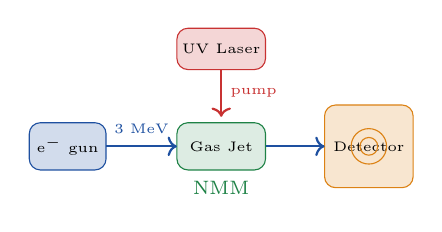
\begin{tikzpicture}[scale=0.75, every node/.style={font=\tiny}]
        % Laser
        \draw[fill=scired!20, draw=scired, rounded corners] (0,2.5) rectangle (1.5,3.2);
        \node at (0.75,2.85) {UV Laser};
        \draw[->,scired,thick] (0.75,2.5) -- (0.75,1.7);
        \node[scired] at (1.3,2.1) {pump};

        % Gas jet
        \draw[fill=scigreen!15, draw=scigreen, rounded corners] (0,0.8) rectangle (1.5,1.6);
        \node at (0.75,1.2) {Gas Jet};
        \node[scigreen] at (0.75,0.5) {\scriptsize NMM};

        % Electron beam
        \draw[fill=sciblue!20, draw=sciblue, rounded corners] (-2.5,0.8) rectangle (-1.2,1.6);
        \node at (-1.85,1.2) {e$^-$ gun};
        \draw[->,sciblue,thick] (-1.2,1.2) -- (0,1.2);
        \node[sciblue] at (-0.6,1.5) {3 MeV};

        % Detector
        \draw[fill=sciorange!20, draw=sciorange, rounded corners] (2.5,0.5) rectangle (4,1.9);
        \node at (3.25,1.2) {Detector};
        \draw[->,sciblue,thick] (1.5,1.2) -- (2.5,1.2);

        % Diffraction pattern
        \draw[sciorange] (3.25,1.2) circle (0.3);
        \draw[sciorange] (3.25,1.2) circle (0.15);
      \end{tikzpicture}
    \end{block}

    \begin{exampleblock}{关键优势}
      \scriptsize
      \begin{itemize}
        \item 直接测量\textbf{原子间距离}（非光谱间接推断）
        \item 适用于气相有机分子光化学研究
        \item 与光电子能谱互补
      \end{itemize}
    \end{exampleblock}
  \end{columns}
\end{frame}

% Slide 4: 泵浦-探测实验流程
\begin{frame}{泵浦-探测实验流程}
  \begin{columns}[T]
    \column{0.55\textwidth}
    \begin{block}{实验流程}
      \scriptsize
      \begin{enumerate}
        \item \textbf{泵浦}：$\sim$200\,nm UV激光脉冲激发NMM分子 $\to$ Rydberg态
        \item \textbf{探测}：延迟 $\Delta t$ 后，MeV电子束散射
        \item \textbf{采集}：45个时间延迟点（$-370$ 至 $+1606$\,fs）
        \item \textbf{统计}：240次实验 $\to$ 200次bootstrap重采样
      \end{enumerate}
    \end{block}

    \begin{block}{数据特征}
      \scriptsize
      \begin{itemize}
        \item 散射信号：637个$s$点，$s = 0.012$--$15.6\anginv$
        \item 9个pre-pump帧（$t<0$）作为基态参考
        \item 信噪比：$s > 9\anginv$时SNR $< 1$
      \end{itemize}
    \end{block}

    \column{0.42\textwidth}
    \begin{block}{时间延迟分布}
      \scriptsize
      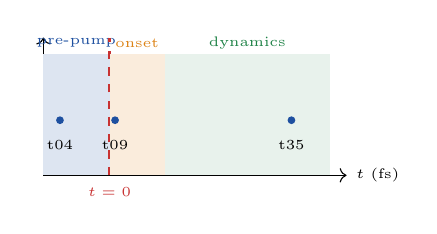
\begin{tikzpicture}[scale=0.7]
        \draw[->] (0,0) -- (5.5,0) node[right] {\tiny $t$ (fs)};
        \draw[->] (0,0) -- (0,2.5);
        % pre-pump region
        \fill[sciblue!15] (0,0) rectangle (1.2,2.2);
        \node[sciblue,font=\tiny] at (0.6,2.4) {pre-pump};
        % time zero
        \draw[scired,thick,dashed] (1.2,0) -- (1.2,2.5);
        \node[scired,font=\tiny] at (1.2,-0.3) {$t=0$};
        % pump onset
        \fill[sciorange!15] (1.2,0) rectangle (2.2,2.2);
        \node[sciorange,font=\tiny,text width=1cm,align=center] at (1.7,2.4) {onset};
        % late time
        \fill[scigreen!10] (2.2,0) rectangle (5.2,2.2);
        \node[scigreen,font=\tiny] at (3.7,2.4) {dynamics};
        % markers
        \foreach \x/\l in {0.3/t04, 1.3/t09, 4.5/t35} {
          \fill[sciblue] (\x,1) circle (2pt);
          \node[font=\tiny,below] at (\x,0.8) {\l};
        }
      \end{tikzpicture}
    \end{block}

    \begin{alertblock}{核心挑战}
      \scriptsize
      从 $\dsm(s)$ 反演原子间距离是\textbf{不适定问题}：
      \begin{itemize}
        \item 信号是距离的正弦变换之和
        \item 噪声导致反演不唯一
        \item 传统方法需要先验结构模型
      \end{itemize}
    \end{alertblock}
  \end{columns}
\end{frame}

% Slide 5: NMM 分子
\begin{frame}{NMM 分子：结构与光化学}
  \begin{columns}[T]
    \column{0.50\textwidth}
    \begin{block}{N-Methylmorpholine (NMM, C$_5$H$_{11}$NO)}
      \scriptsize
      \begin{itemize}
        \item 六元含氮含氧杂环（morpholine骨架 + N-甲基）
        \item 基态N为\textbf{sp$^3$锥形}（pyramidal）
        \item 7个重原子：C1, C2, N3, C4, C5(甲基), C6, O7
        \item 11个H原子锁死在母体重原子上
      \end{itemize}
    \end{block}

    \begin{block}{NMM 分子结构}
      \scriptsize
      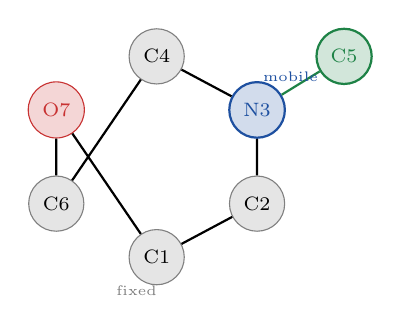
\begin{tikzpicture}[scale=0.85, every node/.style={font=\scriptsize}]
        % Ring atoms
        \node[circle,draw=gray,fill=gray!20,minimum size=14pt] (C1) at (0,0) {C1};
        \node[circle,draw=gray,fill=gray!20,minimum size=14pt] (C2) at (1.5,0.8) {C2};
        \node[circle,draw=sciblue,fill=sciblue!20,minimum size=14pt,thick] (N3) at (1.5,2.2) {\textcolor{sciblue}{N3}};
        \node[circle,draw=gray,fill=gray!20,minimum size=14pt] (C4) at (0,3.0) {C4};
        \node[circle,draw=gray,fill=gray!20,minimum size=14pt] (C6) at (-1.5,0.8) {C6};
        \node[circle,draw=scired,fill=scired!20,minimum size=14pt] (O7) at (-1.5,2.2) {\textcolor{scired}{O7}};
        % Methyl
        \node[circle,draw=scigreen,fill=scigreen!20,minimum size=14pt,thick] (C5) at (2.8,3.0) {\textcolor{scigreen}{C5}};
        % Bonds
        \draw[thick] (C1)--(C2) (C2)--(N3) (N3)--(C4) (C4)--(C6) (C6)--(O7) (O7)--(C1);
        \draw[thick,scigreen] (N3)--(C5);
        % Labels
        \node[gray,font=\tiny] at (-0.3,-0.5) {fixed};
        \node[sciblue,font=\tiny] at (2.0,2.7) {mobile};
      \end{tikzpicture}
    \end{block}

    \column{0.46\textwidth}
    \begin{block}{光化学动力学}
      \scriptsize
      \begin{itemize}
        \item UV激发（$\sim$200--230\,nm）$\to$ 3s/3p Rydberg态
        \item 触发\textbf{氮伞模振动}（umbrella mode）
        \item 振动周期 $\sim$650\,fs
        \item Franck-Condon位移 $\sim$17°
        \item 相干振荡在 $\sim$750\,fs退相干
      \end{itemize}
    \end{block}

    \begin{exampleblock}{研究意义}
      \scriptsize
      \begin{itemize}
        \item 首次从UED数据\textbf{直接测量}伞模振幅（\AA 尺度）
        \item 将光谱学角度位移转化为实际原子间距变化
        \item 含氮杂环光化学的模型体系
      \end{itemize}
    \end{exampleblock}

    \begin{alertblock}{关键距离}
      \scriptsize
      \renewcommand{\arraystretch}{1.05}
      \begin{tabular}{@{}lcl@{}}
        \toprule
        距离 & 平衡值(\AA) & 物理意义 \\
        \midrule
        O-N & 2.851 & 环内对角 \\
        O-C5 & 4.222 & 甲基到O \\
        N-C5 & 1.455 & N-甲基键 \\
        \bottomrule
      \end{tabular}
    \end{alertblock}
  \end{columns}
\end{frame}

% Slide 6: 挑战
\begin{frame}{挑战：散射信号反演的不适定性}
  \begin{columns}[T]
    \column{0.50\textwidth}
    \begin{block}{正问题 vs 逆问题}
      \scriptsize
      \textbf{正问题}（已知结构 $\to$ 信号）：
      \begin{equation*}
        sM(s) = s \sum_{i<j} 2f_i f_j \frac{\sin(s\,r_{ij})}{r_{ij}} \bigg/ \sum_k f_k^2
      \end{equation*}
      解析、唯一、可快速计算

      \vspace{4pt}
      \textbf{逆问题}（信号 $\to$ 距离）：
      \begin{itemize}
        \item 非线性、不适定
        \item 噪声放大
        \item 多组距离可产生相似信号
      \end{itemize}
    \end{block}

    \begin{alertblock}{传统方法的局限}
      \scriptsize
      \begin{itemize}
        \item 需要先验反应坐标模型
        \item 迭代拟合耗时（分钟/帧）
        \item 参数空间探索不充分
        \item 不确定性量化困难
      \end{itemize}
    \end{alertblock}

    \column{0.46\textwidth}
    \begin{block}{域偏差问题}
      \scriptsize
      合成训练信号 $\neq$ 实验信号：
      \begin{itemize}
        \item \textbf{噪声量级}：实验噪声 $\gg$ 理论预期
        \item \textbf{散射模型}：IAM近似 vs 真实电子密度
        \item \textbf{仪器效应}：探测器非均匀性、背景散射
      \end{itemize}
    \end{block}

    \begin{exampleblock}{ML方案的优势}
      \scriptsize
      \begin{itemize}
        \item \textbf{无需先验}：不假设反应坐标
        \item \textbf{快速}：$<1$\,ms/帧
        \item \textbf{不确定性}：bootstrap自然传播
        \item \textbf{灵活}：更换分子只需重新生成训练集
      \end{itemize}
    \end{exampleblock}

    \begin{block}{关键创新}
      \scriptsize
      噪声匹配训练 + DPWA散射因子 + 7维标签设计
    \end{block}
  \end{columns}
\end{frame}

% Slide 7: 方案概述
\begin{frame}{方案概述：ML 回归 Pipeline}
  \begin{center}
    \begin{tikzpicture}[
      node distance=0.6cm,
      box/.style={draw=sciblue, fill=sciblue!10, rounded corners, minimum width=2.5cm, minimum height=0.7cm, font=\scriptsize, align=center},
      arrow/.style={->,>=stealth,thick,sciblue},
      label/.style={font=\tiny,sciblue},
      scale=0.9, transform shape
    ]
      % Training pipeline (top)
      \node[box] (sample) {分子构型采样\\N3圆柱 + C5球体};
      \node[box, right=of sample] (signal) {计算$\dsm(s)$\\DPWA散射因子};
      \node[box, right=of signal] (noise) {添加噪声\\匹配实验噪底};
      \node[box, right=of noise] (train) {训练CNN\\NMMRegressorV2};

      \draw[arrow] (sample) -- (signal);
      \draw[arrow] (signal) -- (noise);
      \draw[arrow] (noise) -- (train);

      \node[above=0.2cm of signal,font=\scriptsize\bfseries,sciblue] {训练阶段};

      % Inference pipeline (bottom)
      \node[box, below=1.5cm of sample] (exp) {实验$\dsm(s,t)$\\200 bootstrap};
      \node[box, right=of exp] (preproc) {预处理\\参考减除+基线校正};
      \node[box, right=of preproc] (infer) {模型推理\\$<1$\,ms/帧};
      \node[box, right=of infer] (recon) {3D结构重建\\三球交点算法};

      \draw[arrow] (exp) -- (preproc);
      \draw[arrow] (preproc) -- (infer);
      \draw[arrow] (infer) -- (recon);

      \node[above=0.2cm of preproc,font=\scriptsize\bfseries,scired] {推理阶段};

      % Connect training to inference
      \draw[arrow,dashed,scired] (train) -- ++(0,-0.9) -| (infer);
    \end{tikzpicture}
  \end{center}

  \vspace{4pt}
  \begin{columns}[T]
    \column{0.32\textwidth}
    \begin{block}{输入}
      \scriptsize
      681点 $\dsm(s)$ 信号\\
      $s \in [0, 15]\anginv$
    \end{block}
    \column{0.32\textwidth}
    \begin{block}{输出}
      \scriptsize
      7个原子间距离(\AA)\\
      O-N, O-C5, N-C5, N-C2,\\N-C4, C5-C2, C5-C4
    \end{block}
    \column{0.32\textwidth}
    \begin{block}{验证}
      \scriptsize
      key\_mae = 0.0966\,\AA\\
      overall\_mae = 0.1479\,\AA
    \end{block}
  \end{columns}
\end{frame}

% =====================================================================
\section{方法论}

% Slide 8: 分子模型
\begin{frame}{分子模型：固定/移动原子}
  \begin{columns}[T]
    \column{0.50\textwidth}
    \begin{block}{自由度设计}
      \scriptsize
      \begin{itemize}
        \item \textbf{固定原子}（5个）：C1, C2, C4, C6, O7
        \item 保持基态DFT优化坐标（B3LYP/6-311++G**）
        \item \textbf{移动原子}（2个）：N3, C5
        \item 光激发主要驱动N3伞模运动和C5甲基随动
        \item \textbf{H原子}（11个）：锁死在母体重原子上
        \item 参与散射计算但不提供额外自由度
      \end{itemize}
    \end{block}

    \begin{exampleblock}{物理依据}
      \scriptsize
      \begin{itemize}
        \item Rydberg态主要改变N的锥度（sp$^3 \to$ sp$^2$）
        \item O和平面C原子在激发态变化极小
        \item H原子C-H键长/角度几乎不变
      \end{itemize}
    \end{exampleblock}

    \column{0.46\textwidth}
    \begin{block}{基态坐标(\AA)}
      \scriptsize
      \renewcommand{\arraystretch}{1.05}
      \begin{tabular}{@{}lrrr@{}}
        \toprule
        原子 & $x$ & $y$ & $z$ \\
        \midrule
        C1 & 1.174 & $-$0.215 & $-$1.143 \\
        C2 & 1.201 & 0.192 & 0.327 \\
        \textcolor{sciblue}{N3} & \textcolor{sciblue}{0.000} & \textcolor{sciblue}{$-$0.296} & \textcolor{sciblue}{1.005} \\
        C4 & $-$1.201 & 0.192 & 0.327 \\
        \textcolor{scigreen}{C5} & \textcolor{scigreen}{0.000} & \textcolor{scigreen}{0.022} & \textcolor{scigreen}{2.424} \\
        C6 & $-$1.174 & $-$0.215 & $-$1.143 \\
        O7 & 0.000 & 0.264 & $-$1.791 \\
        \bottomrule
      \end{tabular}
    \end{block}

    \begin{block}{H原子绑定}
      \scriptsize
      \begin{tabular}{@{}lc@{}}
        C1, C2, C4, C6 & 各2个H \\
        C5 (甲基) & 3个H \\
        N3, O7 & 无H \\
      \end{tabular}

      总计：7重原子 + 11\,H = 18原子
    \end{block}
  \end{columns}
\end{frame}

% Slide 9: 采样策略
\begin{frame}{采样策略：N3 圆柱 + C5 球体}
  \begin{columns}[T]
    \column{0.50\textwidth}
    \begin{block}{N3 采样（圆柱约束）}
      \scriptsize
      \begin{itemize}
        \item 以基态N3坐标为中心
        \item 圆柱半径 $R_N = 2.0\AAng$
        \item 离面偏移 $d_\perp = 2.0\AAng$
        \item 面积均匀采样：$r \sim \sqrt{U(0, R_N^2)}$
        \item 方位角 $\theta \sim U(0, 2\pi)$
      \end{itemize}
    \end{block}

    \begin{block}{C5 采样（球体约束）}
      \scriptsize
      \begin{itemize}
        \item 以基态C5坐标为中心
        \item 球体半径 $R_{C5} = 3.0\AAng$
        \item 体积均匀采样：$r \sim (U(0,R^3))^{1/3}$
        \item 方向角：$\cos\theta \sim U(-1,1)$, $\phi \sim U(0,2\pi)$
      \end{itemize}
    \end{block}

    \column{0.46\textwidth}
    \begin{block}{约束条件}
      \scriptsize
      采样后验证：$r_{N\text{-}O} < r_{C5\text{-}O}$

      违反则\textbf{丢弃重采样}

      接受率 $\approx 68\%$
    \end{block}

    \begin{exampleblock}{近平衡态增强}
      \scriptsize
      \texttt{equil\_fraction = 0.3}：30\%的训练样本从基态小扰动生成

      \begin{itemize}
        \item 高斯扰动 $\sigma = 0.1\AAng$ (N3, C5)
        \item 确保Franck-Condon区域充分采样
        \item 改善pre-pump预测精度
      \end{itemize}
    \end{exampleblock}

    \begin{block}{采样参数演进}
      \scriptsize
      \renewcommand{\arraystretch}{1.05}
      \begin{tabular}{@{}lcc@{}}
        \toprule
        参数 & 初始 & 当前 \\
        \midrule
        $R_N$ & 3.5\,\AA & \textbf{2.0\,\AA} \\
        $R_{C5}$ & 5.0\,\AA & \textbf{3.0\,\AA} \\
        equil\_frac & 0 & \textbf{0.3} \\
        \bottomrule
      \end{tabular}

      缩小范围 $\to$ 提高采样密度 $\to$ 降低MAE
    \end{block}
  \end{columns}
\end{frame}

% Slide 10: 信号计算
\begin{frame}{信号计算：IAM + $\dsm$}
  \begin{columns}[T]
    \column{0.50\textwidth}
    \begin{block}{独立原子模型（IAM）}
      \scriptsize
      原子散射：
      \begin{equation*}
        I_A(s) = \sum_i |f_i(s)|^2
      \end{equation*}
      分子干涉：
      \begin{equation*}
        I_M(s) = \sum_{i<j} 2 f_i(s) f_j(s) \frac{\sin(s\,r_{ij})}{s\,r_{ij}}
      \end{equation*}
      修正散射强度：
      \begin{equation*}
        sM(s) = \frac{s \cdot I_M(s)}{I_A(s)}
      \end{equation*}
    \end{block}

    \begin{block}{差分信号}
      \scriptsize
      训练信号 = 激发态信号 $-$ 基态信号：
      \begin{equation*}
        \dsm_{\text{train}}(s) = sM(s;\text{struct}) - sM(s;\text{equil})
      \end{equation*}
      与实验 $\dsm = sM(t) - \overline{sM}(t<0)$ 约定一致
    \end{block}

    \column{0.46\textwidth}
    \begin{block}{DPWA 散射因子}
      \scriptsize
      \begin{itemize}
        \item 使用相对论\textbf{Dirac partial-wave analysis}散射因子
        \item 来源：\texttt{params/DPWA/fC.mat, fH.mat, fN.mat, fO.mat}
        \item 680点，$s = 0.022$--$15.0\anginv$
        \item 插值到681点模型网格
        \item 归一化：$f_C(s \to 0) = Z_C = 6$
      \end{itemize}
    \end{block}

    \begin{block}{信号特征}
      \scriptsize
      \begin{itemize}
        \item 有效范围：$s \in [1.0, 12.0]\anginv$
        \item 低$s$：受非弹性背景影响
        \item 高$s$：信噪比急剧下降
        \item 18个原子 $\to$ $\binom{18}{2} = 153$个原子对
        \item 信号是所有原子对贡献的\textbf{叠加}
      \end{itemize}
    \end{block}
  \end{columns}
\end{frame}

% Slide 11: 噪声模型
\begin{frame}{噪声模型与数据增强}
  \begin{columns}[T]
    \column{0.50\textwidth}
    \begin{block}{三层噪声模型}
      \scriptsize
      \textbf{1. 高斯白噪声}（主要）
      \begin{itemize}
        \item $\sigma \sim U[0.002, 0.02]$
        \item 随$s$衰减：$\sigma(s) = \sigma_0 / (s + 0.5)$
        \item 模拟光子计数统计噪声
      \end{itemize}

      \textbf{2. 低频漂移}
      \begin{itemize}
        \item $\sigma_{\text{drift}} \sim U[0, 0.01]$
        \item 31点移动平均平滑
        \item 模拟仪器慢漂
      \end{itemize}

      \textbf{3. 尖峰噪声}（可选，当前关闭）
      \begin{itemize}
        \item 概率 $p = 0.002$，幅度 $\sigma = 0.2$
        \item 模拟探测器坏点
      \end{itemize}
    \end{block}

    \column{0.46\textwidth}
    \begin{block}{噪声匹配策略}
      \scriptsize
      \begin{itemize}
        \item 早期模型（低噪声）在实验数据上\textbf{完全失败}
        \item 实验噪底 $\approx 27\times$ 理论预期
        \item \textbf{关键发现}：训练噪声必须匹配实验噪底
        \item 从pre-pump bootstrap方差提取噪声特征
      \end{itemize}
    \end{block}

    \begin{exampleblock}{数据增强}
      \scriptsize
      \begin{itemize}
        \item 每个样本独立随机噪声
        \item 等效于无限数据增强
        \item 近平衡态样本（equil\_fraction=0.3）
        \item \textbf{计划}：Mixup增强（$\alpha=0.2$）
      \end{itemize}
    \end{exampleblock}
  \end{columns}
\end{frame}

% Slide 12: 网络架构
\begin{frame}{网络架构：NMMRegressorV2}
  \begin{center}
    \begin{tikzpicture}[
      node distance=0.35cm,
      block/.style={draw=sciblue, fill=sciblue!10, rounded corners, minimum width=1.8cm, minimum height=0.5cm, font=\tiny, align=center},
      arrow/.style={->,>=stealth,sciblue,thick},
      scale=0.85, transform shape
    ]
      % Input
      \node[block,fill=scigray] (input) {输入\\(B, 1, 681)};

      % Multi-scale stem
      \node[block, right=0.6cm of input] (b3) {Conv1d\\$k$=3};
      \node[block, above=0.1cm of b3] (b7) {Conv1d\\$k$=7};
      \node[block, below=0.1cm of b3] (b15) {Conv1d\\$k$=15};
      \node[block, below=0.1cm of b15] (b31) {Conv1d\\$k$=31};

      \draw[arrow] (input) -- (b3);
      \draw[arrow] (input) |- (b7);
      \draw[arrow] (input) |- (b15);
      \draw[arrow] (input) |- (b31);

      % Concat + BN
      \node[block, right=0.6cm of b3, minimum height=1.8cm] (concat) {Concat\\BN+GELU\\Conv1d(1)\\$C$=128};
      \draw[arrow] (b7.east) -| ($(concat.west)+(0,0.4)$);
      \draw[arrow] (b3) -- (concat);
      \draw[arrow] (b15.east) -| ($(concat.west)+(0,-0.4)$);
      \draw[arrow] (b31.east) -| ($(concat.west)+(0,-0.7)$);

      % Residual blocks
      \node[block, right=0.5cm of concat, minimum width=2.2cm] (res) {8$\times$ ResBlockV2\\BN-GELU-Conv-BN\\-GELU-Conv + SE\\MaxPool@3,6};
      \draw[arrow] (concat) -- (res);

      % Head
      \node[block, right=0.5cm of res, minimum width=1.8cm] (head) {GAP $\to$ FC(512)\\GELU $\to$ FC(256)\\GELU $\to$ Linear(7)};
      \draw[arrow] (res) -- (head);

      % Output
      \node[block,fill=sciorange!15, right=0.5cm of head] (output) {输出\\(B, 7)\\7个距离};
      \draw[arrow] (head) -- (output);

      % Labels
      \node[above=0.3cm of b7,font=\tiny\bfseries,sciblue] {Multi-Scale Stem};
      \node[above=0.3cm of res,font=\tiny\bfseries,sciblue] {Residual Body};
      \node[above=0.3cm of head,font=\tiny\bfseries,sciblue] {Regression Head};
    \end{tikzpicture}
  \end{center}

  \vspace{2pt}
  \begin{columns}[T]
    \column{0.32\textwidth}
    \begin{block}{多尺度Stem}
      \scriptsize
      4种kernel ($k$=3,7,15,31)\\
      捕获不同空间频率\\
      对应不同距离的原子对
    \end{block}
    \column{0.32\textwidth}
    \begin{block}{SE注意力}
      \scriptsize
      Squeeze-and-Excitation\\
      通道自适应加权\\
      自动聚焦信息丰富通道
    \end{block}
    \column{0.32\textwidth}
    \begin{block}{模型规模}
      \scriptsize
      参数量：\textbf{2,125,831}\\
      $C$=128, 8个残差块\\
      2次MaxPool下采样
    \end{block}
  \end{columns}
\end{frame}

% Slide 13: 训练协议
\begin{frame}{训练协议：AdamW + Cosine + Weighted SmoothL1}
  \begin{columns}[T]
    \column{0.50\textwidth}
    \begin{block}{优化器与调度}
      \scriptsize
      \begin{itemize}
        \item \textbf{优化器}：AdamW, $\eta_0 = 1.5 \times 10^{-4}$, weight decay $= 10^{-4}$
        \item \textbf{Warmup}：3 epochs线性升温
        \item \textbf{调度}：Cosine annealing $\to$ 0, 共50 epochs
        \item \textbf{梯度裁剪}：max norm = 1.0
        \item \textbf{早停}：patience = 15（基于val MAE）
        \item \textbf{批大小}：128
      \end{itemize}
    \end{block}

    \begin{block}{加权损失函数}
      \scriptsize
      \begin{equation*}
        \mathcal{L} = \frac{1}{N} \sum_i \sum_d w_d \cdot \text{SmoothL1}(\hat{y}_{i,d}, y_{i,d})
      \end{equation*}
      权重（7维）：
      \begin{equation*}
        \mathbf{w} = [1.0, 1.0, 2.5, 1.5, 1.5, 3.0, 3.0]
      \end{equation*}

      C5-C2/C5-C4加权3.0（改善C5重建）
    \end{block}

    \column{0.46\textwidth}
    \begin{block}{硬件与耗时}
      \scriptsize
      \begin{tabular}{@{}lr@{}}
        \toprule
        项目 & 配置 \\
        \midrule
        硬件 & Apple M2/M3 (MPS) \\
        训练时长 & $\sim$8\,hr (80K) \\
        每epoch & $\sim$6\,min \\
        推理速度 & $<$1\,ms/帧 \\
        \bottomrule
      \end{tabular}
    \end{block}

    \begin{block}{断点续训}
      \scriptsize
      \begin{itemize}
        \item 每epoch保存resume checkpoint
        \item 包含optimizer/scheduler/epoch/patience状态
        \item \texttt{--resume ckpt.resume.pt} 接续训练
      \end{itemize}
    \end{block}

    \begin{exampleblock}{计划优化}
      \scriptsize
      \begin{itemize}
        \item Combined loss: $0.7 \times$ SmoothL1 $+ 0.3 \times$ MSE
        \item Mixup增强：$\lambda \sim \text{Beta}(0.2, 0.2)$
        \item 100K数据集
      \end{itemize}
    \end{exampleblock}
  \end{columns}
\end{frame}

% Slide 14: 7维标签设计
\begin{frame}{7 维标签设计：为何 3 维不够}
  \begin{columns}[T]
    \column{0.50\textwidth}
    \begin{block}{3维标签的问题}
      \scriptsize
      Phase 1使用3维：[O-N, O-C5, N-C5]

      \begin{itemize}
        \item 验证集 key\_mae = \textbf{0.0809}\,\AA（很好）
        \item 但3个距离不足以唯一确定N3和C5的3D坐标
        \item N3有6个自由度，C5有6个，共12个
        \item 3个距离 $<$ 6个独立约束 $\to$ \textbf{几何模糊}
        \item 实验推理时N-C5距离\textbf{不可靠}
      \end{itemize}
    \end{block}

    \begin{alertblock}{3维的几何模糊性}
      \scriptsize
      给定3个距离(O-N, O-C5, N-C5)，N3和C5在空间中有
      \textbf{无穷多}满足条件的位置（一个环形轨迹）

      $\to$ 无法唯一重建3D结构
    \end{alertblock}

    \column{0.46\textwidth}
    \begin{block}{7维标签设计}
      \scriptsize
      增加到固定锚点C2/C4的距离：

      \renewcommand{\arraystretch}{1.1}
      \begin{tabular}{@{}clc@{}}
        \toprule
        维度 & 距离 & 平衡值(\AA) \\
        \midrule
        1 & O-N & 2.851 \\
        2 & O-C5 & 4.222 \\
        3 & N-C5 & 1.455 \\
        \midrule
        4 & \textcolor{sciblue}{N-C2} & \textcolor{sciblue}{1.462} \\
        5 & \textcolor{sciblue}{N-C4} & \textcolor{sciblue}{1.462} \\
        6 & \textcolor{scigreen}{C5-C2} & \textcolor{scigreen}{2.422} \\
        7 & \textcolor{scigreen}{C5-C4} & \textcolor{scigreen}{2.422} \\
        \bottomrule
      \end{tabular}
    \end{block}

    \begin{exampleblock}{7维的优势}
      \scriptsize
      \begin{itemize}
        \item 7个距离 $>$ 6个DOF $\to$ \textbf{过约束}
        \item 可唯一确定N3+C5的3D坐标
        \item 支持三球交点（trilateration）重建
        \item 额外约束提供\textbf{自洽性检验}
      \end{itemize}
    \end{exampleblock}
  \end{columns}
\end{frame}

% =====================================================================
\section{阶段性成果}

% Slide 15: Phase 1 结果
\begin{frame}{Phase 1 结果：3-dim 模型}
  \begin{columns}[T]
    \column{0.50\textwidth}
    \begin{block}{模型配置}
      \scriptsize
      \begin{tabular}{@{}lr@{}}
        \toprule
        参数 & 值 \\
        \midrule
        标签维度 & 3 (O-N, O-C5, N-C5) \\
        训练数据 & 80,000 \\
        验证数据 & 8,000 \\
        equil\_fraction & 0.0 \\
        散射因子 & DPWA \\
        训练epoch & 40 \\
        \bottomrule
      \end{tabular}
    \end{block}

    \begin{exampleblock}{验证集性能}
      \scriptsize
      \begin{tabular}{@{}lc@{}}
        \toprule
        距离 & MAE (\AA) \\
        \midrule
        O-N & 0.0504 \\
        O-C5 & 0.1230 \\
        N-C5 & 0.0693 \\
        \midrule
        \textbf{key\_mae} & \textbf{0.0809} \\
        \bottomrule
      \end{tabular}
    \end{exampleblock}

    \column{0.46\textwidth}
    \begin{alertblock}{实验推理问题}
      \scriptsize
      \begin{itemize}
        \item O-N预测合理，pre-pump接近平衡值
        \item O-C5有偏移但趋势可信
        \item \textbf{N-C5预测不可靠}：波动大、物理上不合理
        \item 原因：3个距离信息不足，模型学到的是\textbf{统计捷径}
      \end{itemize}
    \end{alertblock}

    \begin{block}{关键教训}
      \scriptsize
      \begin{enumerate}
        \item 验证集MAE好 $\neq$ 实验数据好
        \item 需要更多距离约束消除几何模糊
        \item $\to$ 升级到7维标签
      \end{enumerate}
    \end{block}
  \end{columns}
\end{frame}

% Slide 16-17: Phase 2 结果
\begin{frame}{Phase 2 结果：7-dim 模型}
  \begin{columns}[T]
    \column{0.50\textwidth}
    \begin{block}{模型配置变更}
      \scriptsize
      \begin{tabular}{@{}lcc@{}}
        \toprule
        参数 & Phase 1 & Phase 2 \\
        \midrule
        标签维度 & 3 & \textbf{7} \\
        equil\_fraction & 0.0 & \textbf{0.3} \\
        损失权重 & [1,1,2] & [1,1,2,1.5,1.5,2,2] \\
        $R_N$ & 3.5\,\AA & \textbf{2.0\,\AA} \\
        $R_{C5}$ & 5.0\,\AA & \textbf{3.0\,\AA} \\
        \bottomrule
      \end{tabular}
    \end{block}

    \begin{exampleblock}{7-dim eq 验证集性能}
      \scriptsize
      \begin{tabular}{@{}lc@{}}
        \toprule
        距离 & MAE (\AA) \\
        \midrule
        O-N & 0.0519 \\
        O-C5 & 0.1187 \\
        N-C5 & 0.1191 \\
        N-C2 & 0.0813 \\
        N-C4 & 0.0708 \\
        C5-C2 & 0.2179 \\
        C5-C4 & 0.2155 \\
        \midrule
        \textbf{key\_mae} & \textbf{0.0966} \\
        \textbf{overall\_mae} & \textbf{0.1479} \\
        \bottomrule
      \end{tabular}
    \end{exampleblock}

    \column{0.46\textwidth}
    \begin{block}{改善}
      \scriptsize
      \begin{itemize}
        \item 7维提供足够约束进行\textbf{3D重建}
        \item 所有key距离MAE $< 0.12$\,\AA
        \item N-C2/N-C4: 0.07--0.08\,\AA（优秀）
      \end{itemize}
    \end{block}

    \begin{alertblock}{仍存在的问题}
      \scriptsize
      \begin{itemize}
        \item C5-C2/C5-C4 MAE $\approx 0.22$\,\AA（较高）
        \item 实验推理：pre-pump偏差 $\sim$14--18\%
        \item 域偏差仍是主要瓶颈
      \end{itemize}
    \end{alertblock}

    \begin{block}{零输入测试}
      \scriptsize
      输入全零信号 $\to$ 预测应接近平衡值

      结果：所有维度偏差 $\leq \pm 3.4\%$

      $\to$ 模型对基态有良好的先验
    \end{block}
  \end{columns}
\end{frame}

% Slide 18: 训练曲线对比
\begin{frame}{训练曲线对比}
  \begin{columns}[T]
    \column{0.50\textwidth}
    \begin{block}{三代模型训练对比}
      \scriptsize
      \begin{itemize}
        \item \textbf{3-dim 80K}：收敛最快，key\_mae最低
        \item \textbf{7-dim 80K}：增加维度后MAE略升
        \item \textbf{7-dim 80K eq}：equil\_fraction=0.3，pre-pump改善
      \end{itemize}
    \end{block}

    \begin{block}{实际训练图}
      \scriptsize
      \begin{center}
        \textit{[训练曲线图: results/training/]}

        左图：train loss vs val loss（同轴）

        右图：per-distance MAE vs epoch
      \end{center}
    \end{block}

    \column{0.46\textwidth}
    \begin{block}{关键指标演进}
      \scriptsize
      \renewcommand{\arraystretch}{1.1}
      \begin{tabular}{@{}lccc@{}}
        \toprule
        指标 & 3d & 7d & 7d\_eq \\
        \midrule
        key\_mae & \textbf{0.081} & 0.093 & 0.097 \\
        overall & --- & 0.125 & \textbf{0.148} \\
        pre-pump偏差 & 大 & 中 & \textbf{小} \\
        可重建3D & 否 & 是 & \textbf{是} \\
        \bottomrule
      \end{tabular}
    \end{block}

    \begin{exampleblock}{equil\_fraction的效果}
      \scriptsize
      \begin{itemize}
        \item 零输入偏差：从$\sim$10\% 降至 $\leq$3.4\%
        \item Pre-pump预测稳定性显著提高
        \item 代价：overall MAE略升（训练分布更集中）
      \end{itemize}
    \end{exampleblock}
  \end{columns}
\end{frame}

% Slide 19: 验证散点图
\begin{frame}{验证散点图 + 误差分析}
  \begin{columns}[T]
    \column{0.50\textwidth}
    \begin{block}{Parity Plots}
      \scriptsize
      \begin{center}
        \textit{[7维 pred vs true 散点图]}

        \textit{[results/validation/parity\_plots\_7dim\_eq.png]}
      \end{center}
      \begin{itemize}
        \item 对角线 = 完美预测
        \item 密度热力图显示预测分布
        \item 标注MAE和$R^2$
      \end{itemize}
    \end{block}

    \column{0.46\textwidth}
    \begin{block}{误差分析}
      \scriptsize
      \begin{center}
        \textit{[误差直方图 + 相关矩阵]}

        \textit{[results/validation/error\_analysis\_7dim\_eq.png]}
      \end{center}
      \begin{itemize}
        \item 误差直方图：近似对称、无系统偏差
        \item C5-C2/C5-C4误差高度相关（共享C5）
        \item 误差vs真值：远离平衡态时误差增大（异方差）
      \end{itemize}
    \end{block}
  \end{columns}

  \vspace{4pt}
  \begin{block}{误差分析关键发现}
    \scriptsize
    \begin{itemize}
      \item O-N和N-C2/N-C4预测最准确（$R^2 > 0.95$）
      \item C5-C2/C5-C4误差最大——C5位置的不确定性
      \item 误差在极端构型（远离平衡态）时增大——需要更密集的边界采样或数据增强
    \end{itemize}
  \end{block}
\end{frame}

% Slide 20: 实验推理
\begin{frame}{实验推理：时间分辨距离轨迹}
  \begin{columns}[T]
    \column{0.50\textwidth}
    \begin{block}{推理配置}
      \scriptsize
      \begin{tabular}{@{}lr@{}}
        \toprule
        参数 & 值 \\
        \midrule
        模型 & nmm\_v2\_7dim\_80k\_eq \\
        信号模式 & ΔsM (delta) \\
        Alpha & \textbf{0.02} (网格搜索优化) \\
        Bootstrap & 200次均值 \\
        时间点 & 45 ($-$370 -- +1606\,fs) \\
        s范围 & [1.5, 9.0]\,$\text{\AA}^{-1}$ \\
        基线校正 & 2阶多项式, $s > 5.0$ \\
        \bottomrule
      \end{tabular}
    \end{block}

    \begin{block}{推理结果}
      \scriptsize
      \begin{center}
        \textit{[时间分辨距离图]}

        \textit{[results/inference/inference\_7dim\_80k\_eq\_errbar.png]}
      \end{center}
    \end{block}

    \column{0.46\textwidth}
    \begin{block}{关键观测}
      \scriptsize
      \begin{itemize}
        \item \textbf{Pre-pump}（$t<0$）：平均偏差\textbf{5.7\%}
        \item O-N仅偏\textbf{0.2\%}，O-C5偏1.2\%
        \item \textbf{泵浦后}：O-N增加\textbf{+0.45\,\AA}（16\%）
        \item O-C5缩短$-$0.31\,\AA，N-C2/C4增加$+$0.3--0.4\,\AA
        \item 最大O-N位移在$t \approx 134$\,fs
      \end{itemize}
    \end{block}

    \begin{exampleblock}{Alpha优化结果}
      \scriptsize
      \begin{itemize}
        \item 网格搜索$\alpha \in [0.02, 0.04]$
        \item 最优$\alpha = 0.02$：偏差8.6\% $\to$ \textbf{5.7\%}
        \item O-N从2.3\%降至\textbf{0.2\%}
      \end{itemize}
    \end{exampleblock}
  \end{columns}
\end{frame}

% =====================================================================
\section{结构重建}

% Slide 21: 三球交点重建算法
\begin{frame}{三球交点重建算法}
  \begin{columns}[T]
    \column{0.50\textwidth}
    \begin{block}{重建原理}
      \scriptsize
      已知3个锚点（O7, C2, C4）和3个距离 $\to$ 三球交点

      \textbf{N3定位}：
      \begin{itemize}
        \item 锚点：O7, C2, C4
        \item 距离：$d_{ON}$, $d_{NC2}$, $d_{NC4}$
        \item 求解得2个镜像解
      \end{itemize}

      \textbf{C5定位}：
      \begin{itemize}
        \item 锚点：O7, C2, C4
        \item 距离：$d_{OC5}$, $d_{C5C2}$, $d_{C5C4}$
        \item 求解得2个镜像解
      \end{itemize}
    \end{block}

    \begin{block}{解的选择}
      \scriptsize
      $2 \times 2 = 4$种组合，选使
      $|d_{NC5}^{\text{recon}} - d_{NC5}^{\text{pred}}|$ 最小的组合

      $d_{NC5}$作为\textbf{第7个约束}消解镜像模糊
    \end{block}

    \column{0.46\textwidth}
    \begin{block}{算法}
      \scriptsize
      经典trilateration：
      \begin{enumerate}
        \item 建立以$P_1$为原点的局部坐标系
        \item 在局部坐标下解二次方程
        \item 得到 $h = \sqrt{r_1^2 - x^2 - y^2}$
        \item 两个解：$P \pm h\hat{e}_z$
      \end{enumerate}
    \end{block}

    \begin{exampleblock}{重建成功率}
      \scriptsize
      \begin{itemize}
        \item 合成数据：\textbf{100\%}成功
        \item 实验数据（$\alpha$=0.02）：\textbf{45/45}时间点成功
        \item 残差 $< 0.01$\,\AA（几何高度自洽）
      \end{itemize}
    \end{exampleblock}

    \begin{block}{重建自洽性}
      \scriptsize
      重建残差 = $|d_{\text{recon}} - d_{\text{input}}|$

      典型残差 $< 0.01$\,\AA（说明7维距离\textbf{几何自洽}）
    \end{block}
  \end{columns}
\end{frame}

% Slide 22: 3D 结构快照
\begin{frame}{3D 结构重建快照}
  \begin{block}{6个时间点的分子结构快照}
    \scriptsize
    \begin{center}
      \textit{[3D结构快照图：6帧]}

      \textit{[results/reconstruction/structure\_snapshots.png]}
    \end{center}
    \begin{itemize}
      \item 灰色/红色：固定原子（C1,C2,C4,C6,O7）
      \item 蓝色：N3（重建位置）；绿色：C5（重建位置）
      \item $\times$标记：基态平衡位置（对比用）
      \item 虚线：N3-C5键，标注键长
    \end{itemize}
  \end{block}
\end{frame}

% Slide 23: 坐标轨迹
\begin{frame}{N3/C5 坐标轨迹}
  \begin{columns}[T]
    \column{0.50\textwidth}
    \begin{block}{坐标轨迹图}
      \scriptsize
      \begin{center}
        \textit{[N3和C5的XYZ坐标 vs 时间]}

        \textit{[results/reconstruction/coordinate\_trajectories.png]}
      \end{center}
    \end{block}

    \begin{block}{位移量图}
      \scriptsize
      \begin{center}
        \textit{[N3和C5离平衡态的位移 vs 时间]}

        \textit{[results/reconstruction/displacement\_from\_equilibrium.png]}
      \end{center}
    \end{block}

    \column{0.46\textwidth}
    \begin{block}{物理解读}
      \scriptsize
      \begin{itemize}
        \item \textbf{N3 Z轴}：反映伞模振动（锥度变化）
        \item N3从sp$^3$位置向平面运动 $\to$ Z坐标减小
        \item \textbf{C5}：跟随N3运动但幅度较小
        \item Pre-pump：坐标接近平衡值（验证）
      \end{itemize}
    \end{block}

    \begin{exampleblock}{预期vs观测}
      \scriptsize
      \begin{tabular}{@{}lcc@{}}
        \toprule
        特征 & 预期 & 观测 \\
        \midrule
        O-N增加 & $>$0 & \textbf{+0.45\,\AA} \\
        N3 pre偏移 & $<$0.3 & 0.34\,\AA \\
        C5 pre偏移 & $<$0.5 & 0.74\,\AA \\
        最大变化时刻 & --- & $\sim$134\,fs \\
        \bottomrule
      \end{tabular}
    \end{exampleblock}
  \end{columns}
\end{frame}

% =====================================================================
\section{总结与展望}

% Slide 24: 关键结果汇总
\begin{frame}{关键结果汇总}
  \begin{block}{三代模型对比}
    \scriptsize
    \renewcommand{\arraystretch}{1.1}
    \begin{tabular}{@{}lcccc@{}}
      \toprule
      \textbf{模型} & \textbf{key\_mae (\AA)} & \textbf{overall\_mae (\AA)} & \textbf{3D重建} & \textbf{pre-pump偏差} \\
      \midrule
      3-dim 80K & \textbf{0.0809} & --- & 否 & 大 \\
      7-dim 80K & 0.0931 & 0.125 & 是 & 中 \\
      7-dim 80K eq & 0.0966 & 0.148 & 是 & \textbf{小（$\leq$3.4\%）} \\
      \bottomrule
    \end{tabular}
  \end{block}

  \begin{columns}[T]
    \column{0.48\textwidth}
    \begin{exampleblock}{主要成果}
      \scriptsize
      \begin{enumerate}
        \item 建立了从 $\dsm(s) \to$ 7维距离的\textbf{端到端ML pipeline}
        \item 7维标签设计支持\textbf{唯一3D结构重建}
        \item equil\_fraction策略有效改善\textbf{近基态预测}
        \item DPWA散射因子提高物理准确性
        \item Bootstrap不确定性自然传播
      \end{enumerate}
    \end{exampleblock}

    \column{0.48\textwidth}
    \begin{alertblock}{主要局限}
      \scriptsize
      \begin{enumerate}
        \item C5-C2/C5-C4 MAE较高（$\sim$0.22\,\AA）
        \item 实验域偏差导致pre-pump偏移
        \item 训练信号与实验信号的系统性差异
        \item 尚未验证振荡周期与光谱数据的一致性
      \end{enumerate}
    \end{alertblock}
  \end{columns}
\end{frame}

% Slide 25: 局限性与下一步
\begin{frame}{局限性与下一步}
  \begin{columns}[T]
    \column{0.48\textwidth}
    \begin{alertblock}{当前局限}
      \scriptsize
      \begin{enumerate}
        \item \textbf{域偏差}：合成 vs 实验信号系统差异
        \item \textbf{C5精度}：远距离（C5-C2/C5-C4）MAE高
        \item \textbf{单模型}：无集成推理的鲁棒性
        \item \textbf{IAM近似}：忽略化学键电子密度
      \end{enumerate}
    \end{alertblock}

    \begin{block}{域偏差缓解策略（最高优先级）}
      \scriptsize
      \begin{itemize}
        \item \textbf{策略1}：实验噪声profile匹配
        \item 从bootstrap方差提取$s$-dependent噪声
        \item \textbf{策略2}：伪实验数据微调
        \item 合成信号过完整预处理pipeline
        \item \textbf{策略3}：Alpha自动网格搜索
      \end{itemize}
    \end{block}

    \column{0.48\textwidth}
    \begin{exampleblock}{近期优化计划}
      \scriptsize
      \begin{enumerate}
        \item Combined loss + Mixup增强
        \item 100K数据集训练
        \item Alpha敏感性扫描
        \item 集成推理（3-seed平均）
      \end{enumerate}
    \end{exampleblock}

    \begin{block}{长期方向}
      \scriptsize
      \begin{itemize}
        \item Franck-Condon区域强化采样
        \item equil\_fraction $\to$ 0.4--0.5
        \item Boltzmann加权采样
        \item Beyond-IAM散射因子
        \item 推广到其他分子体系
      \end{itemize}
    \end{block}
  \end{columns}
\end{frame}

% Slide 26: 致谢
\begin{frame}{致谢}
  \begin{center}
    \vspace{1cm}
    {\Large\textbf{\color{sciblue} 谢谢！}}

    \vspace{0.8cm}
    \begin{tikzpicture}
      \node[draw=sciblue,fill=sciblue!5,rounded corners,
            text width=10cm,align=center,font=\small,
            inner sep=8pt] {
        \textbf{Machine Learning Inversion of MeV-UED Data}\\
        \textbf{for N-Methylmorpholine}\\[6pt]
        \normalfont\scriptsize
        上海交通大学\quad 激光等离子体教育部重点实验室\\[4pt]
        MeV-UED实验设施\\[4pt]
        项目代码：\texttt{NMM\_ML/}
      };
    \end{tikzpicture}

    \vspace{0.8cm}
    \scriptsize\color{gray}
    2026年3月
  \end{center}
\end{frame}

\end{document}
